\begin{figure}

\begin{subfigure}{\linewidth}

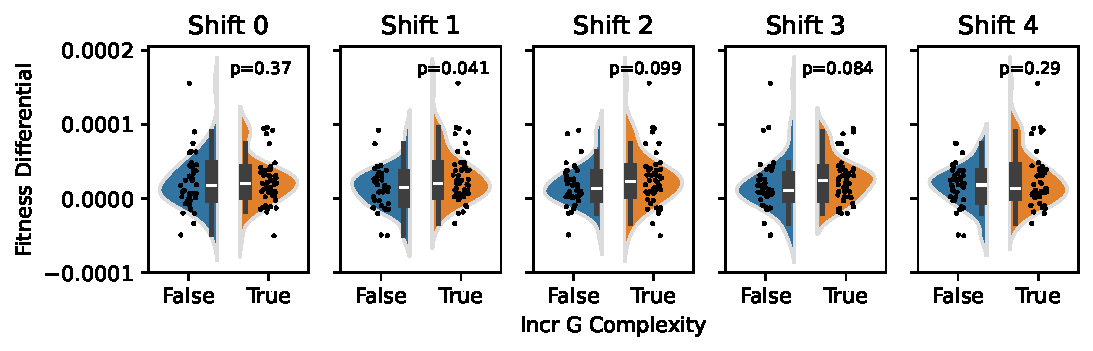
\includegraphics[width=\linewidth]{binder-2025-08-28-complexity-adaptation/binder/teeplots/2025-08-28-complexity-adaptation/how=shift+sign=-1+viz=subplots+ext=.pdf}
\caption{fitness differential value at forward-looking offset, ``shift'' corresponding to offset size}

\end{subfigure}

\vspace{2ex}

\begin{subfigure}{\linewidth}

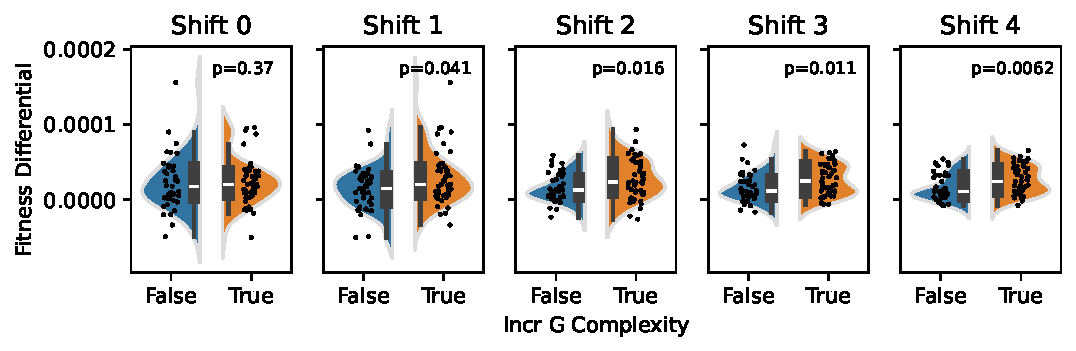
\includegraphics[width=\linewidth]{binder-2025-08-28-complexity-adaptation/binder/teeplots/2025-08-28-complexity-adaptation/how=rollingmean+sign=-1+viz=subplots+ext=.pdf}
\caption{fitness differential mean over forward-looking window, ``shift'' corresponding to window size}

\end{subfigure}

\vspace{1ex}

\caption{
\textbf{Increases in genetic complexity potentiate subsequent fitness gains.}
Split violin plots compare (A) sampled specimens with increased genome complexity relative to their ancestor against (B) sampled specimens with equivalent or decreased genome complexity relative to ancestor.
For specimens with genome complexity increase, no association is detected with population-level fitness gain (shift 0, panel A). However, an association is detected between genome complexity increase and population-level fitness gain within the next sampling window (shift 1, panel A). This effect also appears when measuring mean population-level fitness gains over forward-looking windows.
}
\label{fig:potentiate}

\end{figure}
